% \section{Мотивация}

В столь большом и интересном мире нашлось место и для моей работы,
которая посвящена измерению сечений реакций $e^+e^- \to \pi^0 \gamma$ и
$e^+e^- \to \eta \gamma$ с распадом псевдоскалярного мезона на два
фотона.
Выполняемый анализ проводится по данным набранным детектором КМД-3 на ускорители встречных электрон-позитронных пучков ВЭПП-2000.
Дальнейшая часть реферата пытается показать возможный интерес к
выбранной теме.

\subsection{Относительные вероятности распада}\label{branchings}

Наиболее точные измерения процесса $e^+e^-\to\pi^0\gamma$ проведены в
экспериментах на $e^+e^-$ коллайдере ВЭПП-2М с детекторами КМД-2 и СНД.
Из этих данных только распад $\omega \to \pi^0\gamma$ был измерен с
относительно высокой точностью.

\subsubsection{$\omega \to \pi^0 \gamma$}
\label{omega-to-pi0-gamma}

Точность обобщённого результата КМД-2 и СНД произведения
$B( \omega \to \pi^0 \gamma ) \times B (\omega \to e^+ e^-)$ составляет \SI{1.7}{\percent}.
Однако, это значение произведения отличается от
аналогичного, рассчитанного по $B( \omega \to \pi^0 \gamma )$ и
$B (\omega \to e^+ e^-)$, приведённых в таблице ПДГ \cite{Agashe:2014kda} (см. Рис.~\ref{fig:BweeXBwpig}).
\begin{figure}[htbp]
    \centering
    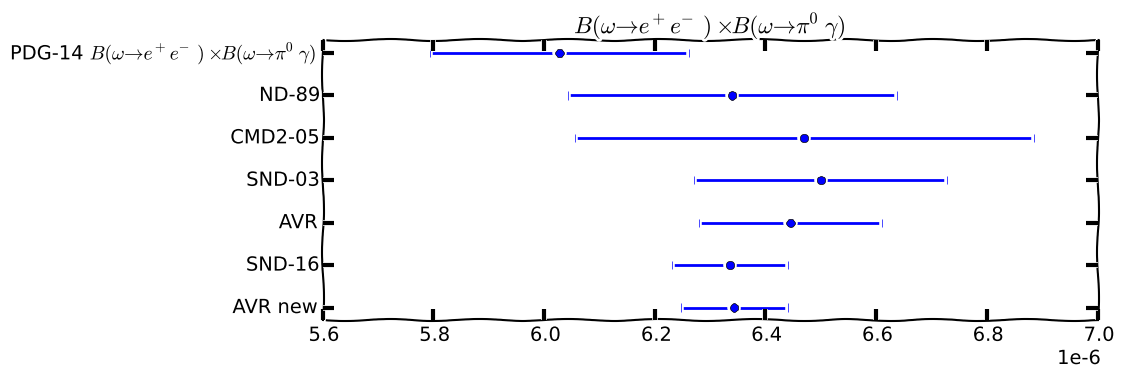
\includegraphics[width=.85\textwidth]{{img/Bw2ee_x_Bwpi0g}.png}
    \caption{$B(\omega \to e^+e^-) \times B(\omega \to \pi^0\gamma)$.
    PDG-14 --- \cite{Agashe:2014kda},
    ND-89 --- \cite{Dolinsky:1988zy},
    CMD2-05 --- \cite{Akhmetshin:2004gw},
    SND-03 --- \cite{Achasov:2003ed},
    AVR --- среднее \cite{Dolinsky:1988zy, Akhmetshin:2004gw, Achasov:2003ed},
    SND-16 --- \cite{Achasov:2016bfr},
    AVR new --- среднее \cite{Dolinsky:1988zy, Akhmetshin:2004gw, Achasov:2016bfr}}
    \label{fig:BweeXBwpig}
\end{figure}
Эта разница вызвана существованием противоречием между измереными значениями
$B( \omega \to \pi^0 \gamma ) \times B(\omega \to e^+ e^-)$,
$B( \omega \to \pi^0 \gamma ) \times B (\omega \to \pi^+ \pi^- \pi^0)$ и
$B( \omega \to \pi^0 \gamma ) / B (\omega \to \pi^+ \pi^- \pi^0)$ (см. Рис.~\ref{fig:Gw2pi0g_o_Gw2pippimpi0}).
Два последних выражения известны с точностью \SI{1.6}{\percent} и \SI{1.8}{\percent} соответственно,
и определяют нынешнее значение $B( \omega \to \pi^0 \gamma )$,
приводимое ПДГ.
Для прояснения этого противоречия необходимо улучшение точности
измерения сечения $e^+e^- \to \pi^0\gamma$ в области $\omega$-резонанса.

\begin{figure}[htbp]
    \centering
    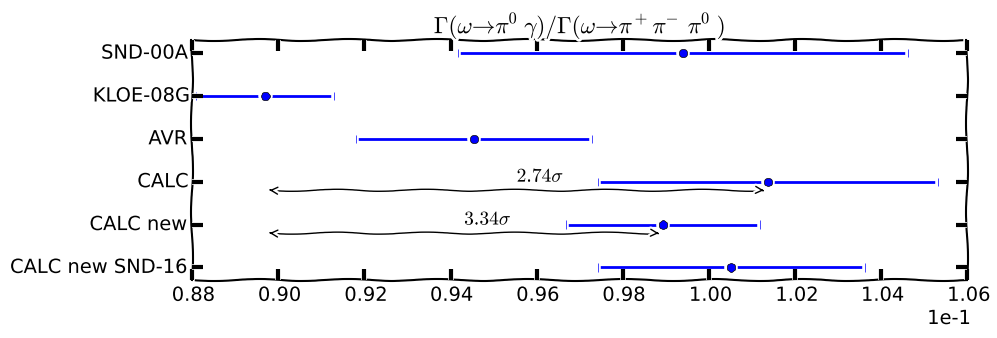
\includegraphics[width=.85\textwidth]{{img/Gw2pi0g_o_Gw2pippimpi0}.png}
    \caption{Отношение ширины распада $\omega \to \pi^0 \gamma$ к $\Gamma (\omega \to \pi^+ \pi^- \pi^0)$.
    SND-00A --- \cite{Aulchenko:2000zq},
    KLOE-08G --- \cite{Ambrosino:2008gb},
    AVR --- средние значение предыдущих двух,
    CALC --- среднее \cite{Akhmetshin:2004gw, Achasov:2003ed, Dolinsky:1988zy} делённое на среднее \cite{Akhmetshin:2003zn, Aubert:2004kj, Achasov:2003ir},
    CALC new --- среднее \cite{Akhmetshin:2004gw, Achasov:2016bfr, Dolinsky:1988zy} делённое на среднее \cite{Akhmetshin:2003zn, Aubert:2004kj, Achasov:2003ir},
    CALC new SND-16 --- \cite{Achasov:2016bfr} делённое на среднее \cite{Akhmetshin:2003zn, Aubert:2004kj, Achasov:2003ir}}
    \label{fig:Gw2pi0g_o_Gw2pippimpi0}
\end{figure}

\subsubsection{\texorpdfstring{$\rho \to \pi^0 \gamma$}{rho --> pi0 gamma}}
\label{rho-to-pi0-gamma}

Точность измерения относительной вероятности распада
$\rho \to \pi^0 \gamma$ составляет \SI{13}{\percent} и определяется статистикой
существующих измерений.

\subsubsection{\texorpdfstring{$\phi \to \pi^0 \gamma$}{}}
\label{phi-to-pi0-gamma}

Формальная точность значения ПДГ вероятности распада
$\phi \to \pi^0 \gamma$ лучше \SI{5}{\percent}.
Оно получено путём усреднения измерений \cite{Achasov:2000zd,Akhmetshin:2004gw} с систематической
ошибкой порядка \SI{8}{\percent} каждое.
Систематическая ошибка возникает из
неопределённости интерференции нерезонансной амплитуды с амплитудой
$\phi \to \pi^0 \gamma$ распада. Нерезонансная амплитуда определяется
вкладами хвостов резонансов $\omega$ и $\rho^0$, заодно дают вклад и
высшие возбуждения векторных мезонов.

Чтобы уменьшить неопределённость таких вкладов, необходимо улучшить
точность измерения сечения $e^+e^- \to \pi^0 \gamma$ в широком диапазоне
энергий от энергий \SI{\sim 300}{\MeVr} до \SI{2}{\GeVr}.

\subsection{Аномальный магнитный момент мюона}\label{mu-amm}

Как люди не могут забыть Герострата, сжёгшего храм Артемиды, так и физики
элементарных частиц рвутся попасть в истории кардинально изменив или
изничтожив современную парадигму науки --- Стандартную Модель. Некоторые
из них ищут Новую Физику пробуя другие области энергии и массы, кто-то
ищет новые распады, другие же могут мерить что-то очень точно и
сравнивать это с предсказаниями теории. К последней группе относится
изучение аномального магнитного момента мюона.

\subsubsection{История}\label{g-2-history}

Экспериментальные измерения $a_\mu$ впервые было осуществлено в СЛАКе \cite{Garwin:1960zz}.
Затем последовала серия измерений в ЦЕРНе, уступившее свое место эксперементу в БНЛ.
В настоящий момент готовится два эксперимента по измерению $g-2$: в ФНАЛ \cite{Grange:2015fou} и Джей-ПАРКе \cite{Saito:2012zz}.

\subsubsection{Вклады в $g-2$}
\label{contribution-to-g-2}

Для нахождения теоретического значения проводятся вычисления.
Традиционно их разбивают на три группы
\begin{equation}
    a_\mu = a_\mu^{QED} + a_\mu^{EW} + a_\mu^{had},
\end{equation}
где $a_\mu^{QED}$ --- электродинамический вклад, $a_\mu^{EW}$ --- вклад
слабых взаимодействий, $a_\mu^{had}$ --- вклад сильных взаимодействий.

Вклад сильных взаимодействий принято разбивать на древесный, с одной
дополнительной вершиной, с двумя и т.\,д.
Отдельно выделяют так называемые
диаграммы рассеяния света на свете.

Изучаемые процессы интересны для всех типов вкладов в $a_\mu^{had}$. 

\subsubsection{Расчёт вкладов в различных
моделях}\label{contribution-calculation}

Существует много способов, чтобы рассчитать те или иные вклады. Главным
образом это вызвано тем, что прямое вычисление согласно КХД крайне
затруднено с математической точки зрения. Для обхода проблемы
используются различные феноменологические модели, а также вычисления на
решётках. Однако, удобнее рассматривать не методы, а научные группы,
которые проводят эти расчёты.


Вклад процессов $\pi^0\gamma$ и $\eta\gamma$ в адронную поляризацию вакуума согласно \cite{Hagiwara:2003da} составляют:
\begin{align}
    a_\mu ( \pi^0 \gamma, 0.6 < \sqrt{s} < \SI{1.03}{\GeVr} ) =
    \num{4.50+-0.15e-10} , \\
    a_\mu ( \pi^0 \gamma, \sqrt{s} < \SI{0.6}{\GeVr} ) =
    \num{0.13+-0.01e-10} , \\
    a_\mu ( \eta \gamma, 0.69 < \sqrt{s} < \SI{1.43}{\GeVr} ) =
    \num{0.73+-0.03e-10} .
\end{align}
Для процесса $\pi^0 \gamma$ в области ниже 0.6 ГэВ отсутствуют экспериментальные данные, вследствии чего сечение реакции экстраполировалось в рамках пертрубативной хиральной теории в приближении доминантности омега-мезона.
В случае процесса $\eta \gamma$ также использовалось ChPT для описания области вблизи порога и был показан вклад менее \num{1e-12}.
Этой же группой в работе \cite{Hagiwara:2011af} для диапазона энергий \SIrange{0.305}{1.8}{\GeVr} были получены значения $a_\mu(\pi^0\gamma) = \num{4.54+-.14e-10}$ и $a_\mu(\eta\gamma) = \num{0.69+-.02e-10}$.

В работе \cite{Ahmadov:2010hq} вычисление вкладов $\eta \gamma$ и $\pi^0 \gamma$ сделано в рамках модели Намбу--Иона-Лазинио с использованием диссперсионного соотношения расчитаны вклады:
\begin{align}
    a_\mu ( \pi^0 \gamma, 0.6 < \sqrt{s} < \SI{1.03}{\GeVr} ) =
    \num{4.5+-0.15e-10} , \\
    a_\mu ( \pi^0 \gamma, \sqrt{s} < \SI{0.6}{\GeVr} ) =
    \num{0.13+-0.01e-10} , \\
    a_\mu ( \eta \gamma, 0.69 < \sqrt{s} < \SI{1.33}{\GeVr} ) =
    \num{0.73+-0.03e-10} ,
\end{align}
полностью соответствующие предыдущим работам.


\subsection{Структура мезонов}
\label{meson-structures}

Являясь частью СМ квантовая хромодинамика отвечает за процессы с участием адронов. Однако, она весьма ограничена в использовании для области энергий с характерной передачей импульса ниже \SI{1}{\GeVr}.
Это привело к популярности феноменологических подходов к описанию физики в данной области энергий.
Используемые модели обладают рядом свободных параметров,
которые можно определять из экспериментальных данных. С другой стороны,
такие модели не только подгоняют уже имеющиеся данные, но обладают
предсказательной силой, величину которой хорошо бы проверять не только качественно, но и числено. Для двух
этих целей --- определение свободных параметров и проверка верности ---
прекрасно подходят сечения изучаемых процессов.
Оба они относятся к магнитным радиационным переходам М1,
что делает их хорошим инструментом для изучения структуры мезонов в
свете различных феноменологических моделей, например кварковой модели с
SU(3) или даже с SU(6) симметрией.

Особый интерес представляют структуры мезонов $\eta$ и $\eta^\prime$, так как в них допускается наличия вкладов $c\bar{c}$-кварков или примесь глюонов. 

В своей статье О'Доннелл \cite{ODonnell:1981sj} исследует кварковый состав мезонов в
рамках кварковой модели и проверяет получаемые результаты с помощью
экспериментальных данных, в то числе, по магнитнодипольным переходам
векторных мезонов в пару фотон-псевдоскаляр.

В статье Болла, Фрере, Титгэт \cite{Ball:1995zv} ках феноменологической модели.% что за модель?
С этой целью рассматриваются радиационные распады
$P \to \gamma \gamma$, $V \to P \gamma$ и $P \to V \gamma$. Упор
делается на работу с основными состояниями, таким образом не учитываются
вклады возбуждённых состояний лёгких векторных мезонов.

Эскрибано и Надаль \cite{Escribano:2007cd} исследовали вклад в глюонов в состояния $\eta$
и $\eta(958)$ провядя феноменологический анализ радиационных распадов
$V (P) \to P (V) \gamma$ в рамках нарушенной SU(3) с учётом
пространственного перекрытия волновых функций $| V \rangle$ и
$|P \rangle$. Авторы заключают, что глюонная составляющая в $\eta$ и
$\eta(958)$ пренебрежимо мала, угол смешивание
$\eta-\eta^\prime = \ang{41.4 \pm 1.3}$, и подчёркивают важность
экспериментальных данных по $(\rho, \omega, \phi ) \to \eta \gamma$ для
проведённых вычислений.

В статье Бенаёун, ДельБуоно, Эйдельмана, Иванченко и О'Коннелла \cite{Benayoun:1999fv} даётся разбор
вопроса о совместном согласованном описании радиационных и лептонных
распадов лёгких мезонов ($V(P) \to P(V)\gamma$, $P \to \gamma \gamma$ и
$V \to e^+ e^-$).


\subsection{Другие измерения}\label{other-measurments}

Данные измерения не будут являться первыми, однако, они возможно смогут
претендовать на сравнимые или улучшенные точности в уже исследованных
областях энергии $\sqrt{s}$ или быть даже первыми и одними из первых в
других. Ниже приведены данные о предыдущих измерениях с целью выявления
современной ситуации в этой области извлечения данных природы.

Сечение процесса $e^+e^-\to\eta\gamma$ исследовалось во многих экспериментах.
Первые опубликованные данные появились в 1976 году из Орсая \cite{Cosme:1975rs}.
Дальнейший поток данных в основном происходит из установок Новосибирска, начиная с работы выполненной на детекторе НД \cite{Druzhinin:1984zq} и продолжая данными с КМД-2 \cite{Akhmetshin:1995vz, Akhmetshin:1999zv, Akhmetshin:2001hm, Akhmetshin:2004gw} и СНД \cite{Achasov:1997nq, Achasov:2000zd, Achasov:2006dv, Achasov:2013eli}.
Также известно измерение сечения реакции на детекторе BaBar \cite{Aubert:2006cy}.

Сечение процесса $e^+e^-\to\pi^0\gamma$ измерено несколько раз, начиная с работы в Орсаи \cite{Cosme:1975rs} и продолжая работами в Новосибирске \cite{Druzhinin:1984zq, Achasov:2000zd, Achasov:2003ed, Akhmetshin:2004gw, Achasov:2016bfr}.